\documentclass[aps,prl,preprint,groupedaddress]{revtex4-1}

\usepackage{amsmath}
\usepackage{amssymb}
\usepackage{mathtools}
\usepackage{listings}
\usepackage{color} %red, green, blue, yellow, cyan, magenta, black, white
\definecolor{mygreen}{RGB}{28,172,0} % color values Red, Green, Blue
\definecolor{mylilas}{RGB}{170,55,241}
\usepackage{blindtext}
\usepackage{fancyvrb}
\usepackage[toc,page]{appendix}
\usepackage{epsfig}
\usepackage[outdir=./]{epstopdf}
\usepackage{graphicx}
\epstopdfsetup{update}
\usepackage{array}

\newcommand{\ba}{\begin{array}}
\newcommand{\ea}{\end{array}}

\newcommand{\bea}{\begin{eqnarray}}
\newcommand{\eea}{\end{eqnarray}}

\newcommand\zt{\stackrel{\mathclap{\normalfont\mbox{ZT}}}{=}}
\newcommand{\bc}{\begin{center}}
\newcommand{\ec}{\end{center}}

\newcommand{\ds}{\displaystyle}

\newcommand{\bt}{\begin{tabular}}
\newcommand{\et}{\end{tabular}}

\newcommand{\bi}{\begin{itemize}}
\newcommand{\ei}{\end{itemize}}

\newcommand{\bd}{\begin{description}}
\newcommand{\ed}{\end{description}}

\newcommand{\bp}{\begin{pmatrix}}
\newcommand{\ep}{\end{pmatrix}}

\newcommand{\pd}{\partial}
\newcommand{\sech}{\mbox{sech}}

\newcommand{\cf}{{\it cf.}~}

\newcommand{\ltwo}{L_{2}(\mathbb{R}^{2})}
\newcommand{\smooth}{C^{\infty}_{0}(\mathbb{R}^{2})}

\newcommand{\br}{{\bf r}}
\newcommand{\bk}{{\bf k}}
\newcommand{\bv}{{\bf v}}

\newcommand{\nidt}{\noindent}

\newcommand{\xbar}{\bar{x}}

\begin{document}
	\author{Matteo Polimeno, Alex Ho}
	\affiliation{Department of Applied Mathematics, UC Merced}
	\date{\today}
	\title{Math232 - Numerical Analysis II\\ Dr. Chrysoula Tsogka\\
		HW1}
\lstset{language=Matlab,%
		%basicstyle=\color{red},
		breaklines=true,%
		morekeywords={matlab2tikz},
		keywordstyle=\color{blue},%
		morekeywords=[2]{1}, keywordstyle=[2]{\color{black}},
		identifierstyle=\color{black},%
		stringstyle=\color{mylilas},
		commentstyle=\color{mygreen},%
		showstringspaces=false,%without this there will be a symbol in the places where there is a space
		numbers=left,%
		numberstyle={\tiny \color{black}},% size of the numbers
		numbersep=9pt, % this defines how far the numbers are from the text
		emph=[1]{for,end,break},emphstyle=[1]\color{red}, %some words to emphasise
		%emph=[2]{word1,word2}, emphstyle=[2]{style},    
}
\maketitle
\section{Problem 1}
\subsection{Part (a)}
Here we are given the data points $\{\bar{x},u(\bar{x})\}$ and $\{\bar{x}+h,u(\bar{x}+h)\}$, and we are going to use them to approximate $u^{\prime}(x)$ using Lagrange Interpolation. Let us define
\begin{align}\label{eq: lag}
U(x) &= u(\xbar)\frac{x-(\xbar+h)}{\xbar-(\xbar+h)}+u(\xbar+h)\frac{x-\xbar}{\xbar+h-\xbar}\nonumber\\
&= u(\xbar)\frac{(x-\xbar-h)}{-h}+u(\xbar+h)\frac{x-\xbar}{h}.
\end{align}
Then, differentiating Eq.~(\ref{eq: lag}) with respect to $x$ yields
\begin{align}\label{eq: dp}
U^{\prime}(x) &= \frac{u(\xbar)}{-h} + \frac{u(\xbar+h)}{h}\nonumber\\
&= \frac{u(\xbar+h)-u(\xbar)}{h}\nonumber\\
&= D_{(+)}u(\xbar)\approx{u^{\prime}(\xbar)},
\end{align}
which is the desired result.
\subsection{Part (b)}
Here we are given the data points $\{\bar{x},u(\bar{x})\}$ and $\{\bar{x}-h,u(\bar{x}-h)\}$, and we are going to use them to approximate $u^{\prime}(x)$ using Lagrange Interpolation. Let us define
\begin{align}\label{eq: lag2}
U(x) &= u(\xbar-h)\frac{x-\xbar}{\xbar-h-\xbar}+u(\xbar)\frac{x-(\xbar-h)}{\xbar-(\xbar-h)}\nonumber\\
&= u(\xbar-h)\frac{x-\xbar}{-h}+u(\xbar)\frac{x-\xbar+h}{h}.
\end{align}
Then, differentiating Eq.~(\ref{eq: lag2}) with respect to $x$ yields
\begin{align}\label{eq: dm}
U^{\prime}(x) &= \frac{u(\xbar)}{h} - \frac{u(\xbar-h)}{h}\nonumber\\
&= \frac{u(\xbar)-u(\xbar-h)}{h}\nonumber\\
&= D_{(-)}u(\xbar)\approx{u^{\prime}(\xbar)},
\end{align}
which is the desired result.
\subsection{Part (c)}
Here we are given the data points $\{\bar{x},u(\bar{x})\}$, $\{\bar{x}+h,u(\bar{x}+h)\}$ and $\{\bar{x}-h,u(\bar{x}-h)\}$, and we are going to use them to approximate $u^{\prime}(x)$ using Lagrange Interpolation. Let us define
\begin{align}\label{eq: lag3}
U(x) &= u(\xbar-h)\frac{(x-\xbar)(x-\xbar-h)}{(\xbar-h-\xbar)(\xbar-h-\xbar-x)}\nonumber\\
&+ u(\xbar)\frac{(x-\xbar-h)(x-\xbar+h)}{(\xbar-\xbar-h)(\xbar-\xbar+h)}\nonumber\\
&+ u(\xbar+h)\frac{(x-\xbar)(x-\xbar+h)}{(\xbar+h-\xbar)(\xbar+h-\xbar+h)}.
\end{align}
Differentiating Eq~(\ref{eq: lag3}) with respect to $x$ yields
\begin{align}
U^{\prime}(x) &= u(\xbar-h)\frac{x-\xbar-h}{2h^{2}}+u(\xbar-h)\frac{x-\xbar}{2h^{2}}+u(\xbar)\frac{x-\xbar+h}{-h^{2}}\nonumber\\
&+u(\xbar)\frac{x-\xbar-h}{-h^{2}}+u(\xbar+h)\frac{x-\xbar}{2h^{2}}+u(\xbar+h)\frac{x-\xbar+h}{2h^{2}}.
\end{align}
At $x=\xbar$ we then have
\begin{align}\label{eq: d0}
U^{\prime}(\xbar) &= \frac{u(\xbar-h)}{-2h}+\frac{u(\xbar)}{-h}+\frac{u(\xbar)}{h}+\frac{u(\xbar+h)}{2h}\nonumber\\
&= \frac{u(\xbar+h)-u(\xbar-h)}{2h}\nonumber\\
&= D_{0}(\xbar)\approx{u^{\prime}(\xbar)}, 
\end{align}
which is the desired result.\\
This particular derivation method does not provide any true quantitative information regarding the local truncation error of the finite differences obtained. It relies on data points, therefore the error is likely inherent to the data-collection process and therefore lies within the data itself. Nevertheless, while we cannot make any quantitative assessment about the error, we can qualitatively compare the different methods. For instance, Eqs.~(\ref{eq: lag}),(\ref{eq: lag2}) are derived using Lagrange Interpolation with two data points, which in fact yields first-degree polynomials in $x$. Taking the derivatives of those first order polynomials at $\xbar$ then gives the scheme in Eqs.~(\ref{eq: dp},\ref{eq: dm}). Therefore, we would expect the order of the error to match the degree of those polynomials (i.e. first order in this case). On the other hand, Eq.~(\ref{eq: lag3}) is derived using Lagrange Interpolation with three data points. We have a second-degree polynomial in $x$, and thus we expect a second-order truncation error. This agrees with what we know from the theory as the Forward and Backward Finite Difference schemes have errors of $\mathcal{O}(h)$, while the Central Finite Difference scheme has error of order $\mathcal{O}(h^{2})$.
\section{Problem 2}
\subsection{Part (a)}
Given
\begin{equation}\label{eq: taylor}
u^{\prime\prime} = c_{-2}u(x-2h)+c_{-1}u(x-h)+c_{0}u(x)+c_{1}u(x+h)+c_{2}u(x+2h)+\mathcal{O}(h^{4}),
\end{equation}
we will use the method of undetermined coefficients to the determine the $c_{i}$'s, $i=-2,..,2$. Let us Taylor expand:
\begin{align*}
u(x-2h) &= u(x)-2hu^{\prime}(x)+2h^2u^{\prime\prime}(x)-\frac{4}{3}h^{3}u^{(3)}(x)+\frac{2}{3}h^{4}u^{(4)}(x)-\frac{32}{120}h^{5}+\mathcal{O}(h^{6}),\\
u(x-h) &= u(x)-hu^{\prime}(x)+\frac{h^2}{2}u^{\prime\prime}(x)-\frac{h^{3}}{6}u^{(3)}(x)+\frac{h^{4}}{24}u^{(4)}(x)-\frac{1}{120}h^{5}+\mathcal{O}(h^{6}),\\
u(x) &= u(x),\\
u(x+h) &= u(x)+hu^{\prime}(x)+\frac{h^2}{2}u^{\prime\prime}(x)+\frac{h^{3}}{6}u^{(3)}(x)+\frac{h^{4}}{24}u^{(4)}(x)+\frac{1}{120}h^{5}+\mathcal{O}(h^{6}),\\
u(x+2h) &= u(x)+2hu^{\prime}(x)+2h^2u^{\prime\prime}(x)+\frac{4}{3}h^{3}u^{(3)}(x)+\frac{2}{3}h^{4}u^{(4)}(x)+\frac{32}{120}h^{5}+\mathcal{O}(h^{6}).\\
\end{align*}
Then, plugging in all these into Eq.~(\ref{eq: taylor}) yields
\begin{align}\label{eq: coeff}
u^{\prime\prime}(x) &= c_{-2}(u(x)-2hu^{\prime}(x)+2h^2u^{\prime\prime}(x)-\frac{4}{3}h^{3}u^{(3)}(x)+\frac{2}{3}h^{4}u^{(4)}(x)-\frac{32}{120}h^{5}+\mathcal{O}(h^{6}))\nonumber\\ &+ c_{-1}(u(x)-hu^{\prime}(x)+\frac{h^2}{2}u^{\prime\prime}(x)-\frac{h^{3}}{6}u^{(3)}(x)+\frac{h^{4}}{24}u^{(4)}(x)-\frac{1}{120}h^{5}+\mathcal{O}(h^{6}))\nonumber\\ &+ c_{0}u(x)\nonumber\\ &+ c_{1}(u(x)+hu^{\prime}(x)+\frac{h^2}{2}u^{\prime\prime}(x)+\frac{h^{3}}{6}u^{(3)}(x)+\frac{h^{4}}{24}u^{(4)}(x)+\frac{1}{120}h^{5}+\mathcal{O}(h^{6}))\nonumber\\ &+ c_{2}(u(x)+2hu^{\prime}(x)+2h^2u^{\prime\prime}(x)+\frac{4}{3}h^{3}u^{(3)}(x)+\frac{2}{3}h^{4}u^{(4)}(x)+\frac{32}{120}h^{5}+\mathcal{O}(h^{6})).
\end{align}
Now, we match the coefficients of same order of derivatives on both sides of Eq.~(\ref{eq: coeff}), simplify and thus build the system
\begin{align*}
c_{-2}+c_{-1}+c_{0}+c_{1}+c_{2}&=0\nonumber\\
-2hc_{-2}-hc_{-1}+hc_{1}+2hc_{2}&=0\nonumber\\
2h^{2}c_{-2}+\frac{h^2}{2}c_{-1}+\frac{h^{2}}{2}c_{1}+2h^{2}c_{2}&=1\nonumber\\
-\frac{4}{3}h^{3}c_{-2}-\frac{h^{3}}{6}c_{-1}+\frac{h^{3}}{6}c_{1}+\frac{4}{3}h^{3}c_{2}&=0\nonumber\\
\frac{2}{3}h^{4}c_{-2}+\frac{h^{4}}{24}c_{-1}+\frac{h^4}{24}c_{1}+\frac{2}{3}h^{4}c_{2}&=0,
\end{align*}
which can be re-written in matrix-vector form as 
\begin{equation}\label{eq: vande}
V{\bf c} = {\bf b},
\end{equation}
where
\[
V=\begin{bmatrix}
1 & 1 & 1 & 1 & 1\\
-2h & -h & 0 & h &2h\\
2h^2 & h^{2}/2 & 0 & h^{2}/2 & 2h^{2}\\
-4h^{3}/3 & -h^{3}{6} & 0 & h^{3}/6 & 4h^{3}/3\\
2h^{4}/3 & h^{4}/24 & 0 & h^{4}/24 & 2h^{4}/3\\ 
\end{bmatrix},~{\bf c}=\begin{bmatrix}
c_{-2}\\
c_{-1}\\
c_{0}\\
c_{1}\\
c_{2}
\end{bmatrix},~{\bf b}=\begin{bmatrix}
0\\
0\\
1\\
0\\
0\\
\end{bmatrix}.
\]
Solving Eq.~(\ref{eq: vande}) in Matlab yields
\[
{\bf c} = \frac{1}{h^{2}}\begin{bmatrix}
-\frac{1}{12}\\
\frac{4}{3}\\
\frac{5}{2}\\
\frac{4}{3}\\
-\frac{1}{12}
\end{bmatrix},
\]
which is in agreement with what we obtained by running the provided Matlab function \textit{fdstencil}.
\subsection{Part(b)}
We include two .txt files (Matlab diary) in CatCourses, with the results obtained by running the provided fdstencil.m in Matlab and the results obtained with the scheme we derived. They match.
\clearpage
\subsection{Part (c)}
Here we are given the function $u(x)=\sin(2x)$ and we are asked to approximate $u^{\prime\prime}(x)$, using the finite difference derived in Part (b), and then compute the error with respect to the true solution. We display our results in Fig.(\ref{fig: err}) and Table \ref{tab: table1}.
\begin{table}
	\begin{tabular}{ |p{4.1cm}||p{4.1cm}|p{4.1cm}| }
		\hline
		\multicolumn{3}{|c|}{Table of the Error for several step-sizes} \\
		\hline
		$h$ & Finite Difference Results & fdcoeffF Results\\
		\hline
		1.0000e-01  & 6.4431e-05 & 6.4431e-05\\
		5.6234e-02  &  6.4588e-06  &  6.4588e-06\\
		3.1623e-02  &    6.4638e-07  &  6.4638e-07\\
		1.7783e-02  &    6.4654e-08  &  6.4655e-08\\
		1.0000e-02  &    6.4612e-09  &  6.4670e-09\\
		5.6234e-03  &    6.5805e-10  &  6.4623e-10\\
		3.1623e-03  &    3.9594e-11  &  6.4150e-11\\
		1.7783e-03  &   -9.2283e-11  & -6.6817e-11\\
		1.0000e-03  &   -2.4144e-10  & -1.8323e-10\\
		5.6234e-04  &   -9.9814e-10  &  -1.8130e-09\\
		3.1623e-04  &   -5.1891e-09  &  4.2406e-09\\
		1.7783e-04  &   -2.0905e-08  &  6.1032e-09\\
		1.0000e-04  &    1.4466e-09  &  -3.8600e-08\\
		\hline
	\end{tabular}
	\caption{\label{tab: table1} Here we look at different step-sizes $h$ (first column), and compare the results obtained in approximating $u(x)=\sin(2x)$ around $x=1$, using the five-point stencils derived in Part (b) (second column) and the provided Matlab Function \textit{fdcoeffF} (third column). As can readily be seen, there is remarkable agreement between the results of the two approaches, therefore we are confident of our analytical derivation.}
\end{table}

\begin{figure}[!htbp]
	\begin{tabular}{c}
		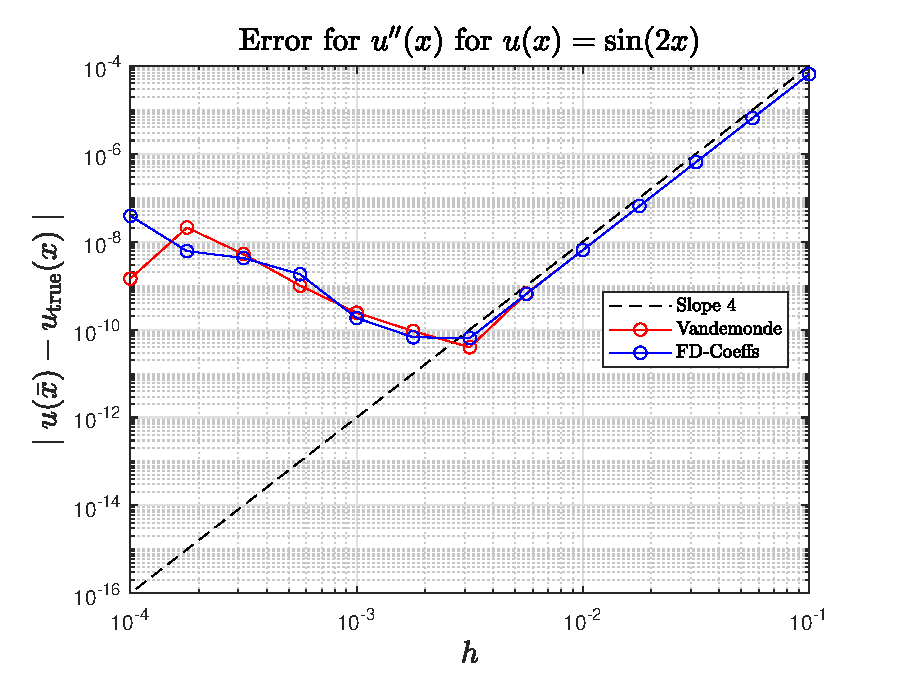
\includegraphics[width=.75\textwidth]{Figures/err_FD}
		(a)\\
	\end{tabular}
	\caption{Plot of the error in a log-log scale. Our Finite Difference scheme (red-line) displays the expected local truncation error of $\mathcal{O}(h^{4})$, for larger values of $h$, as shown by the black line of slope 4. On the other hand, for smaller $h$ values, numerical cancellation of computing $u$ values occurs, impacting the accuracy of the scheme.}
	\label{fig: err}
\end{figure}

\end{document}